% ======================================================================================
%  Scanner-shift OCT benchmark / VLM4RWD — body (rebuilt from reports/oct_format_paper_outline.md)
% ======================================================================================

\begin{abstract}
A glaucoma-OCT reader used across providers should give the same eye the same diagnosis whatever scanner
acquired the image. In practice, however, OCT measurements are not interchangeable across scanners, so a
model's decision can change even though the eye is unchanged. We ask whether prompted frontier vision-language models (VLMs) and specialist OCT foundation models (FMs)
keep a faithful, calibrated decision when the scanner changes. We build a benchmark that applies the scanner change
as a same-eye image transform calibrated to measured cross-scanner disagreement. Because each eye is scored before
and after, the scanner effect is de-confounded from patient differences while the images and labels stay real. We
score the decision at a fixed operating point (a single decision threshold) by its decision-flip rate, change in
sensitivity, and expected calibration error (ECE), with bootstrap confidence intervals (CIs) on the decision metrics. Four results follow.
(1)~Prompted frontier VLMs are the weakest and most overconfident above-chance readers on the raw B-scan (AUC
\num{0.61}--\num{0.69}). Their ECE is roughly 5--10$\times$ the best FM's for the Gemini and GPT families (Claude
Opus~5 a better-calibrated exception); smaller open-weights and medical-specialist VLMs are near chance
(\num{0.41}--\num{0.59}).
(2)~Rendered as a color thickness map, the stronger VLMs reach the level of the strong generic-FM and CNN readers
(AUC \num{0.83}--\num{0.84}), far above their raw-B-scan scores. The small open models do not recover, so what lets a
VLM read the scan is the display format together with a capable base, not model size alone (a cross-dataset
comparison). (3)~A scanner change can break the decision while discrimination is intact:
$\Delta$AUC$\approx$0 while the diagnostic decision flips and specificity can collapse, invisible to AUC-only
evaluation. (4)~Reliability tracks the input representation and pretraining breadth, not model size: across a
26M--197M CNN sweep the largest model is steadiest on neither axis, and on the thickness-map axis a 98k-parameter
from-scratch CNN matches 300M-parameter models on decision stability.
\end{abstract}

% ======================================================================================
\section{Introduction}
\label{sec:intro}

Glaucoma is a leading cause of irreversible blindness, projected to affect 111.8 million people by 2040
\citep{tham2014global} and often undiagnosed \citep{soh2021undetected}. Optical coherence tomography (OCT) of the
retinal nerve fiber layer (RNFL) is a standard
structural test, recommended for diagnosis by clinical practice guidelines \citep{gedde2021ppp}, and deep-learning
readers now detect glaucoma from OCT at the level of specialists \citep{ran2019oct}, increasingly via foundation
models \citep{zhou2023retfound}, producing one decision per eye: glaucoma or not. Prompted frontier vision-language models (VLMs) are being proposed as
general-purpose medical readers \citep{chen2024gmaimmbench, qin2024lmod}, attractive because they do not need task-specific training, but whether they are reliable enough for real deployment is largely untested.

That reliability is tested first by the scanner. Single-site care sidesteps the problem by repetition: the patient is
monitored on one machine and simply re-scanned when referred elsewhere. To meet rising demand
and prevent the follow-up delays that cause avoidable sight loss, clinical guidance is shifting glaucoma care to
virtual, cross-provider triage in which a single digital OCT, acquired in community optometry \citep{jindal2019}, is
shared and read remotely, with AI-assisted coordination \citep{girft2026glaucoma}. Automated readers that support the
decision are increasingly proposed to scale such screening and monitoring across providers
\citep{ting2019ai}, including teleophthalmology \citep{thomas2014teleglaucoma} and multi-site follow-up
\citep{niceng81, gedde2021ppp}. OCT, however, is scanner-dependent: the same eye yields different RNFL measurements
across scanners because segmentation and normative databases differ \citep{buchser2012}, and its raw B-scan
appearance varies with frame-averaging, speckle, and contrast \citep{schmitt1999speckle}. A reader deployed across
providers must therefore treat the scanner as a nuisance variable that does not move the decision: one whose
diagnosis tracks the scanner rather than the eye cannot support multi-provider care, whatever its single-scanner
accuracy.

Single-scanner accuracy cannot see this, and existing work covers only parts of the problem.
Cross-scanner claims for OCT foundation models are made on real cohorts where the scanner coincides with the patient group and are scored by
accuracy or AUC alone \citep{zhou2023retfound, liu2024octcubem, morano2025mirage}. Verbalized-overconfidence studies
use natural images and no clinical decision \citep{groot2024overconfidence}, and medical-VLM trustworthiness
benchmarks span modalities but omit any glaucoma decision under a scanner shift \citep{xia2024cares}. The closest glaucoma
study fine-tunes VLM encoders on a single scanner, with no shift, no decision metric, and no calibration
\citep{jalili2025tvst}. No prior benchmark combines a calibrated same-eye scanner shift, decision-level and
calibration metrics, and a VLM-versus-FM common ground.

We therefore introduce a benchmark that measures this cross-scanner decision reliability directly. We apply the scanner change
as a same-eye image transform calibrated to measured cross-scanner disagreement: published Bland--Altman limits of
agreement for thickness maps \citep{warner2011loa, blandaltman1986} and real per-vendor speckle for B-scans
\citep{schmitt1999speckle, bogunovic2019retouch}. Because the same eye is scored before and after, the scanner effect
is de-confounded from patient differences, and the images and labels stay real. We score
every reader at a fixed operating point by decision-flip, change in sensitivity, and calibration error, with
bootstrap confidence intervals (CIs) on the decision metrics. On this common ground we place prompted frontier VLMs, smaller open-weights and
medical-specialist VLMs, OCT and generic foundation models (FMs), a controlled ImageNet CNN model-size sweep, and a
from-scratch CNN.

\paragraph{Contributions.}
\begin{itemize}[leftmargin=1.2em, itemsep=1pt, topsep=1pt]
\item \textbf{A de-confounded benchmark and decision-level metric suite for scanner-change reliability}
  (\S\ref{sec:benchmark}). To our knowledge the first evaluation that asks whether a glaucoma-OCT reader keeps its
  decision across scanners with the scanner effect isolated from patient differences, scored by a calibration-aware
  metric suite (decision-flip, $\Delta$sens@spec, spec@shift, ECE; bootstrap CIs on the decision metrics) that
  single-scanner accuracy cannot provide, applied uniformly across the VLM, foundation-model, and CNN readers.
\item \textbf{Prompted frontier VLMs are the weakest and most overconfident above-chance readers of raw OCT} (\S\ref{sec:findings},
  F1). On the raw B-scan they fall below the specialist FMs and are badly miscalibrated (with Claude Opus~5 a
  better-calibrated exception), and smaller open-weights and medical-specialist VLMs are near chance, an unsafe
  default for clinical OCT reading.
\item \textbf{Frontier VLMs read a thickness map far better than a raw B-scan} (F2). The stronger frontier VLMs reach
  the strong generic-FM/CNN readers' level on the thickness-map task but fail on the B-scan task, pointing to input
  representation over model size or vendor; the gap is specific to general-purpose VLMs (a cross-dataset comparison we
  caveat in \S\ref{sec:discussion}).
\item \textbf{A scanner change can break the decision while discrimination holds} (F3). Discrimination can be
  unchanged ($\Delta$AUC$\approx$0) while the decision flips and specificity can collapse, a failure AUC-only
  evaluation cannot detect and only decision-level and calibration metrics reveal.
\item \textbf{Stability tracks representation and pretraining breadth, not model size} (F4). Across a one-family CNN
  model-size sweep, OCT and generic FMs, and a from-scratch network, tolerance to the scanner change is flat across
  model size: on the thickness-map axis a 98k-parameter CNN is CI-tied with the best CNNs and matches 300M-parameter models on
  decision stability.
\end{itemize}

% ======================================================================================
\section{Related work}
\label{sec:related}

Three lines of prior work are relevant to our question: the reliability of (medical) VLMs, cross-scanner
generalization of OCT models, and prompted VLMs for glaucoma.

\paragraph{Reliability and evaluation of (medical) VLMs.} Object-hallucination work showed that generative vision
models assert ungrounded content \citep{rohrbach2018chair, li2023pope}. Verbalized-probability elicitation, the
standard cross-model confidence denominator \citep{lin2022verbalized, tian2023calibration, xiong2024uncertainty}, is
weakly calibrated for frontier multimodal models: \citet{groot2024overconfidence} report GPT-4V and Gemini
overconfidence on natural images, in line with the broader result that predictive uncertainty degrades under
dataset shift \citep{ovadia2019shift}. On medical images, general-purpose and medical VLMs (e.g.\ LLaVA-Med
\citep{li2023llavamed}) remain well short of clinical-grade accuracy on broad medical benchmarks
\citep{chen2024gmaimmbench}, reason weakly about eye
images \citep{qin2024lmod}, and on glaucoma reach high accuracy
but poor sensitivity on fundus grading \citep{alryalat2024chatgpt}. Trustworthiness benchmarks such
as CARES score an over-confidence ratio across medical modalities \citep{xia2024cares}. None of these pair a clinical
decision with a calibrated scanner shift and a decision-level, calibration-aware metric, which is our focus.

\paragraph{OCT foundation models and cross-scanner generalization.} OCT-specific foundation models claim cross-scanner
transfer, but on real held-out cohorts where scanner coincides with cohort (a confound) and scored by accuracy or
AUC \citep{zhou2023retfound, liu2024octcubem, morano2025mirage}. A prior mitigation, cross-domain image translation,
can recover device-specific glaucoma-OCT accuracy \citep{belghith2025crossdomain}, but is validated by accuracy on
real cohorts, not by decision stability under a same-eye shift. More broadly, distribution shift, both naturally
occurring \citep{koh2021wilds} and synthetic \citep{hendrycks2019corruptions}, is a mature benchmark topic, and
retinal AI has been externally validated across fundus cameras \citep{tsai2022crosscamera}, the same varying-hardware
design we adopt. We differ by applying the scanner as a calibrated same-eye transform, which de-confounds it from
cohort by construction, and by scoring the decision and its calibration rather than accuracy alone.

\paragraph{Prompted VLMs for glaucoma (the closest neighbor).} \citet{jalili2025tvst} fine-tune VLM vision encoders
on a single scanner and find them competitive with OCT FMs (LLaVA \num{0.92} vs.\ RETFound \num{0.91}), with no
distribution shift, decision metric, or calibration. The same group's GPT-4V study \citep{jalili2024gpt4v} is the
closest prompted-frontier-VLM precedent, but it grades fundus images and reports accuracy only, with no scanner
shift or calibration. Our claim is instead about
\emph{prompted} frontier VLMs (zero- or few-shot, verbalized probability) under a calibrated scanner shift: a
fine-tuned encoder can match a specialist while a prompted generalist stays weak and overconfident, so the two
settings measure different deployment modes.

% ======================================================================================
\section{The benchmark}
\label{sec:benchmark}

\begin{figure}[t]
  \centering
  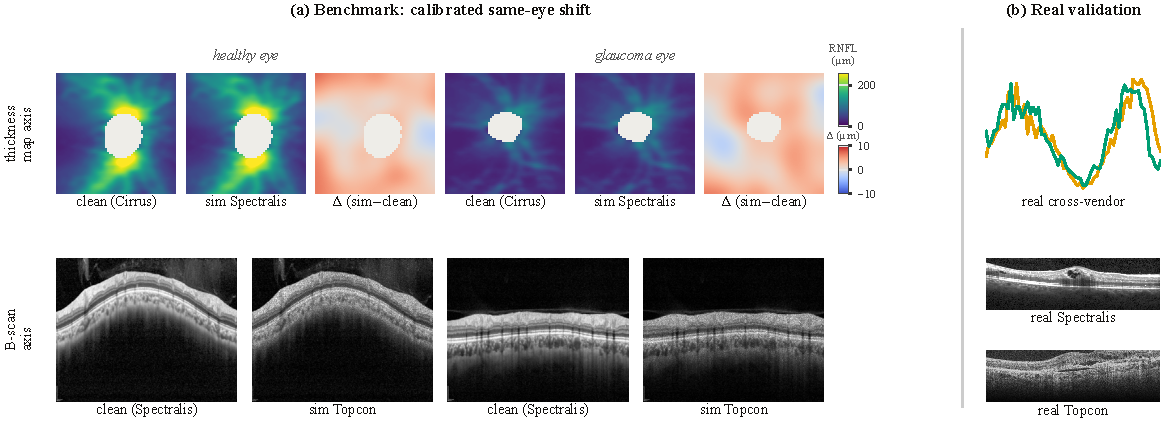
\includegraphics[width=\linewidth]{figures/fig1_overview.pdf}
  \caption{\textbf{The benchmark and its real-data validation.} \textbf{(a)}~The calibrated same-eye shift on
  best-by-eye exemplars. One clear healthy and one clear glaucomatous eye are each shown clean $\rightarrow$ shifted
  on both axes: thickness maps (Harvard-GDP Cirrus, Warner-calibrated Cirrus$\rightarrow$Spectralis; viridis,
  brighter = thicker RNFL) and circumpapillary B-scans (GLEAM Spectralis $\rightarrow$ simulated Topcon). The shift
  is small by design, so each clean/shifted map pair is followed by a difference panel (sim $-$ clean, coolwarm, on a
  shared $\pm10\,\mu$m scale spanning the calibrated LoA), with the largest deviations in the superior and inferior nerve-fiber bundles, where the
  calibrated cross-scanner shift is widest (\S\ref{app:validity}). This is one representative per-eye realization; the
  benchmark applies an independent calibrated shift to every eye. Each reader sees clean and shifted versions of the same eyes, so scanner
  is not confounded with cohort. \textbf{(b)}~Real data corroborating the shift: cross-vendor cpRNFL (circumpapillary RNFL)
  profiles from GLEAM Spectralis and GOALS Topcon agree in shape, and RETOUCH Spectralis/Topcon
  macular B-scans calibrate the per-vendor speckle of the B-scan axis.}
  \label{fig:overview}
\end{figure}

\paragraph{Common-ground harness.} Every reader (a map-reader, an FM linear probe (LP) or fine-tune, or a prompted
VLM) produces the same output: a per-eye glaucoma probability. We score each on paired clean$\rightarrow$shifted
degradation over the same test eyes under the same shared-seed shift, with eye-level percentile-bootstrap 95\% CIs
(2000 resamples; the eye is the unit of analysis; seed-0 split). Each result is labeled by its input
representation, and we never cross-rank across axes.

\paragraph{Two calibrated axes} (Fig.~\ref{fig:overview}; validity in App.~\ref{app:validity}). The two axes span the
three most common OCT vendors (Cirrus, Spectralis, Topcon), which are known not to be interchangeable
\citep{buchser2012}. Each source vendor is fixed by its dataset; we take as the target the pair with a
published calibration anchor (Cirrus$\rightarrow$Spectralis for the thickness map, Spectralis$\rightarrow$Topcon for
the B-scan; App.~\ref{app:validity}). The two axes therefore span two vendor pairs and two shift mechanisms, and the
failure modes recur across both. The two axes are also the two input representations: the color thickness-map and the
raw B-scan, so F2's representation contrast and the two shift axes are the same two settings. \emph{Thickness-map
axis}: Harvard-GDP Cirrus RNFLT maps \citep{luo2023harvardgdp} with labels
($n{=}300$ test, 46\% glaucoma). The shift has three calibrated components: a per-eye bias and limit of agreement
($+1.94\,\mu$m, $\pm7.68\,\mu$m, Warner-calibrated \citep{warner2011loa, blandaltman1986}); a superior/inferior-wider
sector profile from scan-circle centration \citep{cheung2009scancircle}; and a spatially-correlated texture from OCT
segmentation differences \citep{mansberger2017segerrors}. All are matched to real cross-vendor data
(\S\ref{app:validity}). \emph{B-scan axis}: GLEAM \emph{circumpapillary} Spectralis
B-scans \citep{gleam2026} with clinical labels ($n{=}360$ test, 49\% glaucoma). The shift is a Spectralis$\rightarrow$Topcon
appearance stress: a frame-averaging change, injected multiplicative-Gamma speckle, and contrast dimming
\citep{schmitt1999speckle}. Its direction and magnitude are calibrated from real per-vendor RETOUCH macular display
speckle \citep{bogunovic2019retouch}. This axis tests tolerance to appearance changes: its magnitude is
speckle-matched, not bounded by a measured cross-scanner LoA, which would require same-eye disc-OCT on two scanners
that no public dataset provides.

\paragraph{Decision-level metrics.} We report discrimination, decision, and calibration reads; clean AUC, decision-flip, and
$\Delta$sens@spec carry eye-level 95\% bootstrap CIs, and the remaining reads are point estimates. \emph{Discrimination:} clean AUC and $\Delta$AUC (signed clean$-$shift). \emph{Decision:}
decision-\emph{flip} \citep{hendrycks2019corruptions}, the fraction of eyes whose decision (refer / do-not-refer)
changes under the shift; $\Delta$sens@spec, the clean$-$shift change in sensitivity at the operating point; and
\emph{spec@shift}, the specificity actually realized under the shift, which flags a reader that keeps its flip low
only by collapsing specificity. \emph{Calibration:} ECE and $\Delta$ECE \citep{guo2017calibration} over 10
equal-width bins, and the net calibration error (NCE), a signed calibration error \citep{groot2024overconfidence}:
mean predicted-class confidence minus accuracy, so $+$ $=$ overconfident. The operating point is a single threshold fixing 90\% specificity
on clean negatives, applied to shifted scores; fixing it on the clean data makes clean specificity slightly
optimistic, but equally for every reader, so comparisons are unaffected. Because a recalibrating shift leaves
$\Delta$AUC$\approx$0 while the decision flips, it is flip, $\Delta$sens, and spec@shift, not $\Delta$AUC, that reveal the failure.

\paragraph{Readers.} \emph{Frontier closed VLMs} (three developers): Gemini (2.5 Flash, 2.5 Pro, 3.6 Flash),
GPT-5.6 Sol, and Claude Opus~5, zero- and few-shot (k{=}6, single greedy sample; temperature-0 where the API accepts
it, App.~\ref{app:setup}), on both the raw B-scan and a color
thickness-map render. \emph{Open-weights
and specialist VLMs} (self-hosted): Qwen3-VL-8B \citep{qwen3vl2025} and MedGemma-1.5-4B \citep{medgemma15_2026}, same protocol. Elicitation is verbalized
probability \citep{tian2023calibration}: each model states its probability of glaucoma in words rather than reading
it from output logits, the one score common to every vendor, since the closed models expose no
logprobs. \emph{OCT and generic FMs:} RETFound \citep{zhou2023retfound} and MIRAGE \citep{morano2025mirage} against DINOv2 \citep{oquab2023dinov2}, LP and fine-tune.
\emph{ImageNet CNN model-size sweep:} ResNet-50 and ConvNeXt-T/B/L (26M$\rightarrow$197M), frozen probe and
per-architecture fine-tune. \emph{From-scratch:} a 98k-parameter SmallCNN trained end-to-end on each axis.

% ======================================================================================
\section{Experiments and findings}
\label{sec:findings}

We score 29 configurations on the B-scan axis and 25 on the thickness-map axis (the OCT-specific B-scan FMs are not run on map
renders; setup and model/dataset cards in App.~\ref{app:setup}--\ref{app:datasets}). Each finding below states one
claim and gives its eye-level bootstrap-CI evidence; cross-configuration comparisons are descriptive and uncorrected.
Table~\ref{tab:main} lists the headline configurations. Figs.~\ref{fig:stability}--\ref{fig:mechanism} give the
reliability landscape and the shift mechanism.

\begin{table}[t]
  \centering
  \caption{\textbf{Headline configurations, both axes} (calibrated shift, eye-level bootstrap 95\% CIs). Columns: clean AUC,
  decision-\emph{flip}, $\Delta$sens@spec (signed clean$-$shift), clean ECE, net calibration error (NCE) and
  $\Delta$AUC. Lower flip, $|\Delta\text{sens}|$, ECE and $|\Delta\text{AUC}|$ are better. \textbf{Bold} is the best
  AUC, flip and ECE per column among readers with useful discrimination (clean AUC $\ge 0.70$); a near-chance reader
  can post a trivially low flip, so flip is read together with AUC. NCE is a signed calibration error
  \citep{groot2024overconfidence} (mean predicted-class confidence minus accuracy; $+$ $=$ overconfident); $\Delta$sens,
  NCE and $\Delta$AUC are signed diagnostics ($\approx$0 ideal) and are not bolded. The ImageNet-CNN row is the best
  per axis; the from-scratch SmallCNN is trained end-to-end on each axis and never sees the test shift. VLMs are
  prompted (\textit{fs} = few-shot). Full per-axis tables (B-scan 29 configurations, map 25), with realized spec@shift
  and flip/$\Delta$sens CIs, are in App.~\ref{app:fulltables}.}
  \label{tab:main}
  \small
  \renewcommand{\arraystretch}{0.9}
  \setlength{\tabcolsep}{3pt}
  \begin{tabular}{llcccccc}
    \toprule
    Reader & Class & AUC \ci{95\%}{CI} & Flip$\downarrow$ & $\Delta$sens & ECE$\downarrow$ & NCE & $\Delta$AUC \\
    \midrule
    \multicolumn{8}{l}{\textit{\textbf{B-scan axis}} \quad Spectralis\,$\rightarrow$\,Topcon, $n{=}360$ eyes} \\
    \midrule
    DINOv2\,$\cdot$\,FT       & generic FM     & \textbf{0.88} \ci{0.84}{0.91} & \textbf{0.09} & $+0.08$ & 0.05 & $-0.00$ & $+0.01$ \\
    RETFound\,$\cdot$\,FT     & OCT FM         & 0.85 \ci{0.80}{0.89}          & 0.14 & $-0.09$ & 0.07 & $+0.07$ & $-0.01$ \\
    MIRAGE\,$\cdot$\,LP       & OCT FM         & 0.70 \ci{0.65}{0.76}          & 0.47 & $-0.72$ & \textbf{0.04} & $-0.02$ & $+0.04$ \\
    ConvNeXt-B\,$\cdot$\,LP   & ImageNet CNN   & 0.83 \ci{0.78}{0.87}          & 0.11 & $+0.07$ & 0.07 & $+0.03$ & $+0.04$ \\
    SmallCNN (98k)           & scratch CNN    & 0.79 \ci{0.74}{0.83}          & 0.27 & $-0.32$ & \textbf{0.04} & $-0.04$ & $+0.02$ \\
    Gemini 3.6 Flash\,\textit{fs}  & frontier VLM   & 0.69 \ci{0.64}{0.74}          & 0.15 & $+0.01$ & 0.26 & $+0.26$ & $-0.00$ \\
    GPT-5.6 Sol\,\textit{fs}     & frontier VLM   & 0.67 \ci{0.61}{0.73}          & 0.24 & $+0.11$ & 0.23 & $+0.23$ & $-0.01$ \\
    Claude Opus~5\,\textit{fs}& frontier VLM  & 0.67 \ci{0.62}{0.73}          & 0.18 & $+0.05$ & 0.16 & $+0.13$ & $+0.03$ \\
    Qwen3-VL-8B\,\textit{fs} & open VLM       & 0.54 \ci{0.49}{0.58}          & 0.02 & $+0.00$ & 0.38 & $+0.38$ & $+0.00$ \\
    MedGemma-1.5-4B\,\textit{fs}    & specialist VLM & 0.49 \ci{0.43}{0.54}          & 0.00 & $+0.03$ & 0.42 & $+0.42$ & $-0.04$ \\
    \midrule
    \multicolumn{8}{l}{\textit{\textbf{Thickness-map axis}} \quad Cirrus\,$\rightarrow$\,Spectralis, $n{=}300$ eyes} \\
    \midrule
    DINOv2\,$\cdot$\,FT       & generic FM     & \textbf{0.88} \ci{0.83}{0.91} & 0.04 & $+0.01$ & 0.09 & $-0.02$ & $+0.00$ \\
    ConvNeXt-L\,$\cdot$\,FT   & ImageNet CNN   & 0.87 \ci{0.83}{0.91}          & \textbf{0.02} & $+0.01$ & \textbf{0.07} & $-0.04$ & $+0.00$ \\
    SmallCNN (98k)           & scratch CNN    & 0.85 \ci{0.80}{0.89}          & \textbf{0.02} & $+0.00$ & 0.12 & $+0.03$ & $-0.01$ \\
    GPT-5.6 Sol\,\textit{fs}     & frontier VLM   & 0.84 \ci{0.79}{0.88}          & 0.09 & $+0.02$ & 0.11 & $+0.11$ & $-0.00$ \\
    Gemini 3.6 Flash\,\textit{fs}  & frontier VLM   & 0.84 \ci{0.79}{0.88}          & 0.05 & $+0.06$ & 0.15 & $+0.13$ & $+0.02$ \\
    Claude Opus~5\,\textit{fs}& frontier VLM  & 0.83 \ci{0.78}{0.88}          & 0.09 & $+0.03$ & \textbf{0.07} & $+0.01$ & $-0.00$ \\
    Qwen3-VL-8B\,\textit{fs} & open VLM       & 0.59 \ci{0.55}{0.62}          & 0.05 & $+0.00$ & 0.36 & $+0.36$ & $+0.02$ \\
    MedGemma-1.5-4B\,\textit{fs}    & specialist VLM & 0.55 \ci{0.48}{0.61}          & 0.03 & $+0.00$ & 0.30 & $+0.30$ & $+0.02$ \\
    \bottomrule
  \end{tabular}
\end{table}


\begin{figure}[t]
  \centering
  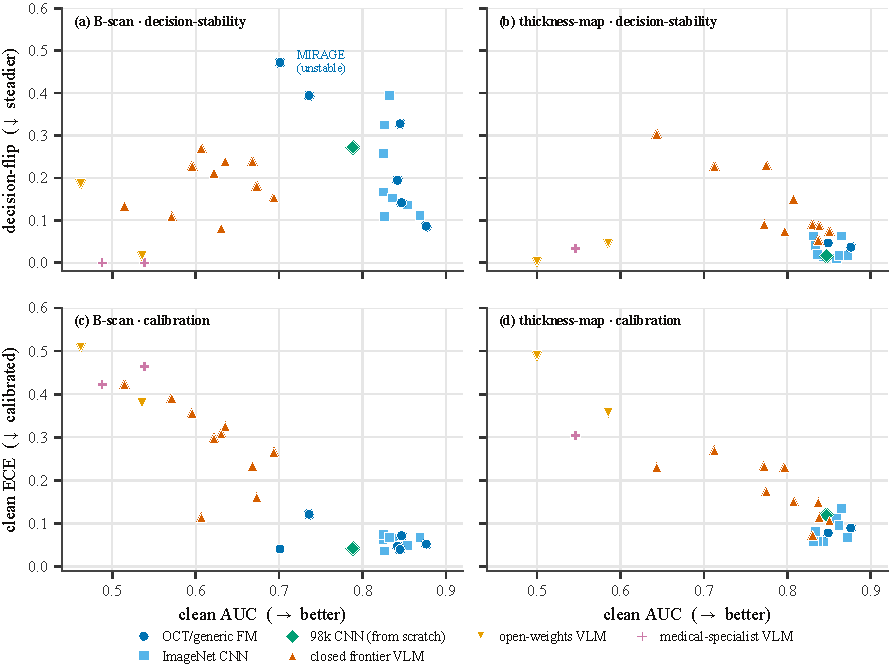
\includegraphics[width=0.9\linewidth]{figures/fig2_stability.pdf}
  \caption{\textbf{Reliability landscape.} Every reader on clean AUC against two reliability metrics,
  \emph{decision-stability} (decision-flip, top row) and \emph{calibration} (clean ECE, bottom row), for the
  B-scan (left) and thickness-map (right) axes. Color and marker encode reader class. Frontier VLMs are
  unstable and overconfident on the raw B-scan (a,c) but recover on the thickness map (b,d); the small open and
  specialist VLMs are near chance on both axes. A $\Delta$AUC$\approx$0 can hide large decision-flips (MIRAGE, panel a), and the
  98k-parameter from-scratch CNN (green diamond) is among the steadiest readers on the thickness-map axis
  (b), CI-tied with the best CNNs, though not steady on the raw B-scan (a).}
  \label{fig:stability}
\end{figure}

\paragraph{F1: prompted frontier VLMs are the weakest and most overconfident above-chance readers, across three developers.}
Among the readers above near-chance, the prompted frontier VLMs rank last. On the raw B-scan, even the best frontier
VLM only matches the weakest specialist's discrimination (MIRAGE\,$\cdot$\,LP, AUC \num{0.70}): Gemini 3.6 Flash few-shot AUC
\num{0.69} \ci{0.64}{0.74}, GPT-5.6 Sol \num{0.67} \ci{0.61}{0.73}, and Claude Opus~5 \num{0.61}/\num{0.67}
(zero/few-shot). The Gemini and GPT configurations are also badly overconfident: their clean (pre-shift) ECE is
\num{0.23}--\num{0.42}, roughly 5--10$\times$ the best FM's \num{0.04}, and their net calibration
error is also large and positive (\num{0.23}--\num{0.42}; per configuration in Table~\ref{tab:main} and
App.~\ref{app:fulltables}), so the miscalibration is overconfidence, not two-sided noise. The gap is not a binning
artifact: it holds under a strictly proper score (Brier) and adaptive-bin ECE, not just fixed-bin ECE
(App.~\ref{app:fulltables}), matches \citet{groot2024overconfidence, xia2024cares}, and is the VLM/FM split in
Fig.~\ref{fig:stability}c. Few-shot lifts discrimination with mixed calibration effect, whereas neither a larger model
nor a higher tier helps (the higher-tier Gemini 2.5 Pro is the worst frontier zero-shot, AUC \num{0.51}). Calibration
is vendor-dependent, with Claude Opus~5 a markedly better exception (ECE \num{0.11}--\num{0.16}). The weakness deepens as models shrink: the open-weights
Qwen3-VL-8B and the specialist MedGemma-1.5-4B are near chance on both axes (AUC \num{0.41}--\num{0.59}) with the highest
ECE (up to \num{0.51}), so neither open weights nor medical-specialist pretraining rescues the decision (the
small-model elicitation caveat in \S\ref{sec:discussion} applies).

\paragraph{F2: general-purpose VLMs read the thickness map, not the raw B-scan.}
On the thickness-map task the same models reach the strong generic-FM/CNN readers' level (DINOv2, ConvNeXt): Gemini
3.6 Flash \num{0.84}, GPT-5.6 Sol \num{0.84} \ci{0.79}{0.88}, and Claude Opus~5 \num{0.83} \ci{0.78}{0.88}. Discrimination,
calibration (ECE roughly halved), and stability (flip dropping) recover together, well above their raw-B-scan level
and across all three developers (per-VLM detail in App.~\ref{app:grounding}). The lift holds even zero-shot (GPT-5.6 Sol \num{0.77} vs.\ \num{0.63}; Claude Opus~5
\num{0.61}$\rightarrow$\num{0.85}), so it is not few-shot memorization, but it needs a capable base: the small open
VLMs do not recover (Qwen3-VL-8B \num{0.50}--\num{0.59}, MedGemma-1.5-4B \num{0.41}--\num{0.55}). The gap is specific to
general-purpose VLMs on the raw B-scan, where reading RNFL requires the implicit segmentation an OCT-trained model
performs while a color thickness map presents thinning directly. A thickness map is not intrinsically a better input
(trained models read glaucoma from raw OCT at least as well \citep{maetschke2019}), and because the two axes use
different datasets this comparison is confounded (\S\ref{sec:discussion}).

\begin{figure}[t]
  \centering
  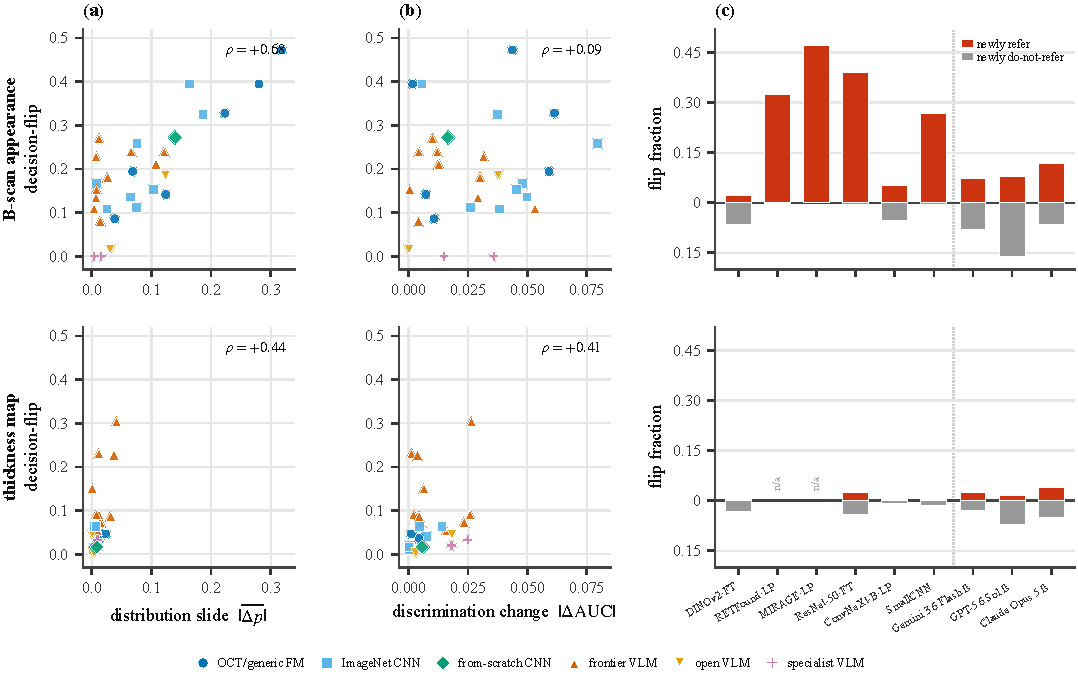
\includegraphics[width=\linewidth]{figures/fig3_mechanism.pdf}
  \caption{\textbf{Decision-flip comes from the score distribution moving, not from a change in discrimination.}
  One row per shift axis (top: B-scan appearance; bottom: thickness map), with matched limits. Across all 29 B-scan
  readers, decision-flip is uncorrelated with the discrimination change $|\Delta\text{AUC}|$ (\textbf{b},
  $\rho{=}0.09$) and rises with the net directional slide $|\overline{\Delta p}|$ (\textbf{a}, $\rho{=}0.68$); readers
  well above the (\textbf{a}) trend (real flip at near-zero net slide) move two-sidedly, and flip tracks the mean
  absolute per-eye movement mean\,$|\Delta p|$ (not plotted) even more tightly ($\rho{=}0.88$). A reader can flip many decisions with its AUC intact. On the
  thickness-map axis (bottom) slide, $|\Delta\text{AUC}|$, and flip are all small.
  \textbf{(c)}~Decision-flip split into newly-``refer'' (over-referral, red) and newly-``do-not-refer'' (grey), for
  representative readers per class plus the frontier VLMs (few-shot; the dotted line separates non-VLM from VLM). The
  appearance-sensitive readers (the OCT FMs MIRAGE\,$\cdot$\,LP and RETFound\,$\cdot$\,LP, the ImageNet
  ResNet-50\,$\cdot$\,FT, and the from-scratch SmallCNN) over-refer almost one-directionally, whereas the generic
  DINOv2\,$\cdot$\,FT and ConvNeXt-B\,$\cdot$\,LP stay robust (small, two-sided). The VLMs flip in
  \emph{model-specific} directions (GPT-5.6 Sol toward do-not-refer, Claude Opus~5 toward refer, Gemini 3.6 Flash either way). The map row (bottom) is
  likewise near-flat for every reader, and the OCT-specific FMs, not run on maps, are marked n/a. Markers in (a,b)
  encode reader class (shared legend).}
  \label{fig:mechanism}
\end{figure}

\paragraph{F3: a scanner change can break the decision while discrimination holds.}
Decision-flip is unrelated to discrimination: across all \num{29} B-scan readers $|\Delta\text{AUC}|\le\num{0.08}$
(about half within \num{0.03}), yet decision-flip spans \num{0.00}--\num{0.47} and shifted specificity \num{0.07}--\num{1.00},
and flip is uncorrelated with $\Delta$AUC (Spearman \num{0.09}). Flip is instead a threshold effect: it rises with the
mean absolute per-eye movement mean\,$|\Delta p|$ (Spearman \num{0.88}; movement $\Delta p =
p_{\text{shift}}-p_{\text{clean}}$) more tightly than with the net directional slide $|\overline{\Delta p}|$
(\num{0.68}; Fig.~\ref{fig:mechanism}a,b), because some readers move their scores two-sidedly and flip without a net
direction. What matters for safety is the direction of the crossings. In the appearance-sensitive readers (the OCT
FMs, the fine-tuned ImageNet CNNs, and the from-scratch SmallCNN) the added speckle pushes scores up, so essentially
every threshold crossing is toward ``refer'' and specificity collapses; the up-shift largely preserves the ordering
of eyes, so AUC holds. MIRAGE\,$\cdot$\,LP is the extreme (all \num{170} flips up, specificity \num{0.07}), with
RETFound\,$\cdot$\,LP ($117/118$ up) and ResNet-50\,$\cdot$\,FT ($140/142$ up) the same, and \num{18}/\num{29} readers
net-shift toward refer (OCT FMs mean $\overline{\Delta p}=+0.24$). This is over-referral, not lost sensitivity
(Fig.~\ref{fig:mechanism}c), and it concentrates on healthy eyes (MIRAGE\,$\cdot$\,LP flips \num{62}\% of healthy
vs.\ \num{28}\% of moderate-to-advanced; no disparity across demographics, underpowered subgroups,
App.~\ref{app:subgroups}). The frontier VLMs and the broadly-pretrained DINOv2 show no such systematic over-referral:
the VLMs flip in model-specific directions (GPT-5.6 Sol toward do-not-refer, Claude Opus~5 toward refer, Gemini 3.6 Flash
either way; flip \num{0.15}--\num{0.24}), and DINOv2 resists ($\overline{\Delta p}=-0.04$), the steadiest capable
reader (flip \num{0.09}). Either way AUC-only evaluation misses the flip while the decision-level metrics expose it.
The thickness-map axis is far more stable ($|\Delta\text{AUC}|\le\num{0.03}$, flip $\le\num{0.31}$).

\paragraph{F4: stability does not track model size; representation and pretraining breadth win.}
Frozen LP clean AUC is unchanged across 26M$\rightarrow$197M (map \num{0.83}--\num{0.84}, B-scan
\num{0.82}--\num{0.83}; CIs overlap), and the largest model is steadiest on neither axis; the color thickness-map is
robust at every size while the raw B-scan is not. Generic DINOv2 is the steadiest and best-discriminating (B-scan
LP$\rightarrow$FT flip \num{0.19}$\rightarrow$\num{0.09}), whereas OCT-specific MIRAGE is weakest (AUC \num{0.70}, flip
\num{0.47}); fine-tuning rescues the other OCT FM (RETFound\,$\cdot$\,FT flip \num{0.14}, AUC \num{0.85}), so the
weakness is MIRAGE-specific, not intrinsic to OCT pretraining, though fine-tuning is no universal fix and can itself
distort features under shift \citep{kumar2022finetuning}. The clearest case is a from-scratch 98k-parameter SmallCNN, trained
end-to-end on the thickness map and never exposed to the test shift: it flips just \num{0.02} \ci{0.00}{0.03} (net
calibration error \num{0.03}), CI-tied with the best ImageNet CNNs and steadier than the 300M DINOv2 (flip
\num{0.04}) at $\sim$900--3000$\times$ fewer parameters, so its stability is a genuine out-of-distribution result
from the compact, task-trained representation, not model size.

% ======================================================================================
\section{Discussion and limitations}
\label{sec:discussion}

\paragraph{What this means for deployment.} Used in a glaucoma-diagnosis pipeline today, a prompted generalist
VLM reading raw B-scans is the least safe above-chance reader: below the specialist FMs and markedly overconfident. But a strong FM or CNN fails differently: it holds its AUC under a
scanner change while its decisions flip, so it passes single-scanner validation and then fails in the field. Where that flip is a specificity collapse, it over-refers the healthy
majority of a screening population (\S\ref{sec:findings}), the costliest place for false referrals. Two things follow. First, this is a decision failure,
not a calibration one: calibration is already poor before any shift and does not significantly worsen under it
($\Delta$ECE CI includes 0), and post-hoc temperature scaling \citep{guo2017calibration} removes most of the clean VLM
ECE (App.~\ref{app:reliability}) yet, being monotonic, leaves the decision-flip unchanged. Second, re-thresholding cannot undo this score movement at
deployment, where no labeled data from the incoming scanner exist, so the remedy is to select readers whose decisions
stay put. The recommendation is concrete: validate a diagnostic reader at its operating point, with calibration and
under a scanner shift, not on single-scanner AUC; our benchmark is that check, and a candidate that flips a quarter of
decisions under a calibrated same-eye shift is unsafe however high its AUC.

\paragraph{What to engineer, and why.} The failure is not fundamental to VLMs. The same models recover to the strong
generic-FM/CNN level once the RNFL is rendered as a readable color thickness map (a cross-dataset contrast; see
\emph{Limitations}). What helps is the input
representation, not model size, vendor, or a ``medical-specialist'' label. The B-scan failure is an appearance
sensitivity, consistent with the added speckle and dimmed contrast being read as RNFL thinning: appearance-keyed readers
(the OCT-specific FMs and fine-tuned CNNs) raise their glaucoma score and over-refer while the broadly-pretrained
generic FM resists (F3--F4); the small open and specialist models recover on neither, so it is an interaction of input format and
capability. Robustness tracks representation and pretraining breadth, not model size: a 98k-parameter task-trained CNN is among
the steadiest readers at $\sim$900--3000$\times$ fewer parameters than the FMs. For practitioners: engineer the input
representation and a compact, task-specific encoder, and require decision stability, not model size, before deployment.

\paragraph{Limitations.} \emph{The same-eye shift is synthetic}: no public same-eye cross-scanner labeled disc-OCT
exists, so we calibrate the shift to published cross-scanner LoA (map) and real per-vendor speckle (appearance) and
keep four datasets real; a real same-eye cross-scanner set is the natural extension. \emph{Elicitation and
calibration are conservative}: VLMs are queried with a single greedy verbalized-probability sample, so the reported
VLM ECE is an upper estimate of overconfidence ($N$-sample, prompt-paraphrase passes are future work); the smallest
open models collapse to a constant (Qwen3-VL-8B on the map), so a boolean-verdict elicitation may be fairer.
\emph{The B-scan-vs-thickness-map comparison (F2) is cross-dataset}: the two axes differ in
dataset, vendor, and labels, so F2 confounds input representation with dataset difficulty and possible
contamination; we read it as reader-specific (\S\ref{sec:findings}), not as evidence a map is better in general.
\emph{Subgroups}: instability is broadly uniform across disease severity and demographics
(App.~\ref{app:subgroups}), but the subgroups are underpowered and image quality is unrecorded, so a definitive
fairness audit needs richer metadata. \emph{Scope}: two axes, never cross-ranked; broader vendor-pair coverage and
extending decision stability to longitudinal progression monitoring are the natural next steps.

% ======================================================================================
\section{Conclusion}
\label{sec:conclusion}

A scanner change can break a glaucoma-OCT reader's decision while its AUC looks unchanged; reliability tracks input
representation and pretraining breadth, not model size. We release our de-confounded, decision-level,
calibration-aware benchmark (four real datasets, only the scanner shift synthesized) as a reusable check, so a
reader's decision stability under a scanner change can be validated before it reaches patients.
